%%%%%%%%%%%%%%%%%%%%%%%%%%%%%%%%%%%%%%%%%%%%%%%%%%%%%%%%
% 							                   PREAMBULE        
%%%%%%%%%%%%%%%%%%%%%%%%%%%%%%%%%%%%%%%%%%%%%%%%%%%%%%%%

\documentclass[a4,12pt]{article}

%--- Packages génériques ---%

\usepackage[francais]{babel}
\usepackage[utf8]{inputenc}
\usepackage[T1]{fontenc}
\usepackage[babel=true]{csquotes}
\usepackage{amsmath}
\usepackage{amssymb}
\usepackage{float}
\usepackage{graphicx}
\usepackage{hyperref}

%--- Structure de la page ---%

\usepackage{fancyheadings}

\topmargin -1.5 cm
\oddsidemargin -0.5 cm
\evensidemargin -0.5 cm
\textwidth 17 cm
\setlength{\headwidth}{\textwidth}
\textheight 24 cm
\pagestyle{fancy}
\lhead[\fancyplain{}{\thepage}]{\fancyplain{}{\sl ENSIMAG 2A}}
\chead[\fancyplain{}{{\sl }}]{\fancyplain{}{{TP Traitement d'Image}}}
\rhead[\fancyplain{}{}]{\fancyplain{}{Loiodice \& Vincent}}
\lfoot{\fancyplain{}{}}
\cfoot{\fancyplain{}{}}
\cfoot{\thepage }
\rfoot{\fancyplain{}{}}

%--- Style de la zone de code ---%

\usepackage{tikz}
\usetikzlibrary{calc}
\usepackage[framemethod=tikz]{mdframed}
\usepackage{listings}             
\usepackage{textcomp}

\lstset{upquote=true,
        columns=flexible,
        keepspaces=true,
        breaklines,
        breakindent=0pt,
        basicstyle=\ttfamily,
        commentstyle=\color[rgb]{0,0.6,0},
        language=Scilab,
        alsoletter=\),
        }

\lstset{classoffset=0,
        keywordstyle=\color{violet!75},
        deletekeywords={zeros,disp},
        classoffset=1,
        keywordstyle=\color{cyan},
        morekeywords={zeros,disp},
        }

\lstset{extendedchars=true,
        literate={0}{{\color{brown!75}0}}1 
                 {1}{{\color{brown!75}1}}1 
                 {2}{{\color{brown!75}2}}1 
                 {3}{{\color{brown!75}3}}1 
                 {4}{{\color{brown!75}4}}1 
                 {5}{{\color{brown!75}5}}1 
                 {6}{{\color{brown!75}6}}1 
                 {7}{{\color{brown!75}7}}1 
                 {8}{{\color{brown!75}8}}1 
                 {9}{{\color{brown!75}9}}1 
                 {(}{{\color{blue!50}(}}1 
                 {)}{{\color{blue!50})}}1 
                 {[}{{\color{blue!50}[}}1 
                 {]}{{\color{blue!50}]}}1
                 {-}{{\color{gray}-}}1
                 {+}{{\color{gray}+}}1
                 {=}{{\color{gray}=}}1
                 {:}{{\color{orange!50!yellow}:}}1
                 {é}{{\'e}}1 
                 {è}{{\`e}}1 
                 {à}{{\`a}}1 
                 {ç}{{\c{c}}}1 
                 {œ}{{\oe}}1 
                 {ù}{{\`u}}1
                 {É}{{\'E}}1 
                 {È}{{\`E}}1 
                 {À}{{\`A}}1 
                 {Ç}{{\c{C}}}1 
                 {Œ}{{\OE}}1 
                 {Ê}{{\^E}}1
                 {ê}{{\^e}}1 
                 {î}{{\^i}}1 
                 {ô}{{\^o}}1 
                 {û}{{\^u}}1 
        }

%--- Raccourcis commande ---%

\newcommand{\R}{\mathbb{R}}
\newcommand{\N}{\mathbb{N}}
\newcommand{\A}{\mathbf{A}}
\newcommand{\B}{\mathbf{B}}
\newcommand{\C}{\mathbf{C}}
\newcommand{\D}{\mathbf{D}}
\newcommand{\ub}{\mathbf{u}}

%--- Mode correction et incréments automatiques ---%

\usepackage{framed}
\usepackage{ifthen}
\usepackage{comment}
\usepackage{graphicx}

\newcounter{Nbquestion}

\newcommand*\question{%
\stepcounter{Nbquestion}%
\textbf{Question \theNbquestion. }}

\newboolean{enseignant}
%\setboolean{enseignant}{true}
\setboolean{enseignant}{false}

\definecolor{shadecolor}{gray}{0.80}

\ifthenelse{
\boolean{enseignant}}{
\newenvironment{correction}{\begin{shaded}}{\end{shaded}}
}
{
\excludecomment{correction}
}

%--- Style de l'encadré des questions ---%

\mdfsetup{leftmargin=12pt}
\mdfsetup{skipabove=\topskip,skipbelow=\topskip}

\tikzset{
	warningsymbol/.style={
	rectangle,draw=red,
	fill=white,scale=1,
	overlay}}
\global\mdfdefinestyle{exampledefault}{
	hidealllines=true,leftline=true,
	innerrightmargin=0.0em,
	innerleftmargin=0.3em,
	leftmargin=0.0em,
	linecolor=red,
	backgroundcolor=orange!20,
	middlelinewidth=4pt,
	innertopmargin=\topskip,
}

\global\mdfdefinestyle{answer}{
	hidealllines=true,leftline=true,
	innerrightmargin=0.0em,
	innerleftmargin=0.3em,
	leftmargin=0.0em,
	linecolor=green,
	backgroundcolor=white,
	middlelinewidth=4pt,
	innertopmargin=\topskip,
}

%%%%%%%%%%%%%%%%%%%%%%%%%%%%%%%%%%%%%%%%%%%%%%%%%%%%%%%%
% 							               EN-TETE        
%%%%%%%%%%%%%%%%%%%%%%%%%%%%%%%%%%%%%%%%%%%%%%%%%%%%%%%%

\title{\textbf{TP2 Traitement d'Image\\Filtrage non linéaire}}
\author{
\begin{tabular}{cc}
	\textsc{Loiodice Thomas} & \textsc{Vincent Kylian} \\
\end{tabular}}   
\date{\small \today}

\makeatletter
	\def\thetitle{\@title}
	\def\theauthor{\@author}
	\def\thedate{\@date}
\makeatother 

\usepackage{etoolbox}
\usepackage{titling}
\setlength{\droptitle}{-7em}

\setlength{\parindent}{1cm}

\makeatletter
% patch pour le bug concernant les parenthèses fermantes d'après http://tex.stackexchange.com/q/69472
\patchcmd{\lsthk@SelectCharTable}{%
  \lst@ifbreaklines\lst@Def{`)}{\lst@breakProcessOther)}\fi}{}{}{}
  
%%%%%%%%%%%%%%%%%%%%%%%%%%%%%%%%%%%%%%%%%%%%%%%%%%%%%%%%
% 							CORPS DU DOCUMENT          
%%%%%%%%%%%%%%%%%%%%%%%%%%%%%%%%%%%%%%%%%%%%%%%%%%%%%%%%

\begin{document}
\maketitle


%%%%%%%%%%%%%%%%%%%%%%%%%%%%%%%%%%%%%%%%%%%%%%%%%%%%%%%%
% 						                  	PARTIE I         
%%%%%%%%%%%%%%%%%%%%%%%%%%%%%%%%%%%%%%%%%%%%%%%%%%%%%%%%

\section{Partie I : Implémentation et estimation des paramètres}
\subsection{Filtre Médian}

\subsection{Filtre Adaptatif Récursif}
Dans le cas de ce filtre, le critère d'arrêt est un élément très important. En effet ce dernier doit être bien défini et estimé pour permettre un filtrage complet sans effectuer d'étapes superflues. Pour cela, l'arrêt est défini sur l'écart (norme 2 sur la différence) entre deux traitements successifs d'images. L'écart seuil a été fixé empiriquement après essais sur les différentes images de test. Nous avons cependant remarqué que le choix du paramètre k de filtrage influe très fortement sur ce critère d'arrêt. En effet, si ce dernier est mal dimmensionné face au niveau de bruit de l'image alors un point fixe est très difficile à atteindre. Dans ce cas l'éxecution est stoppée à 200 itérations, valeur jugée suffisante au regard des essais effectués et de la description du filtre.\\

Dans le cas d'une valeur de $k$ trop importante, les contours se retrouvent découpés trop grossièrement : les bords des formes sont ainsi arrondis et les surfaces des formes internes se voient diminuer.\\

Il n'est pas possible, pour ce filtre, de donner une valeur de K générique fonctionnant de manière optimale pour les différents types et intensités de bruit, K dépendant en effet de ce niveau de bruit. Les valeurs préconisées pour ce paramètre sont comprises entre  10 (faibles bruits) et 50 (forts bruits). Pour trouver ces valeurs nous avons étudié la convergence des images vers un point fixe en affichant la différence entre deux images successives.
\subsection{Filtre Bilatéral}

\subsection{Filtre NL-Means}
Concernant le filtrage NL-Means, l'estimation du meilleur choix de taille de patchs et de région est difficile. En effet le filtre est très coûteux en calculs et rend les tests de différentes valeurs très longs, augmentant avec la taille de ces derniers. Nous avons effectué quelques essais qui nous ont permis d'aboutir à un compromis qui nous a semblé satisfaisant en prenant un taille de patchs \textit{r = 5} et une taille de région \textit{t = 10}. En effet, sur l'exemple de l'image \textit{formes2bb10.pgm} l'écart (de PSNR et visuel) est très faible avec une taille de patchs \textit{r = 5} et une taille de région \textit{t = 15} (\textit{PSNR = 40.01} contre $40.02$ avec les tailles précédentes). Cependant le temps de calcul est, lui, fortement augmenté : respectivement \textit{3m44.028s} (pour \textit{r=5, t=10}) et \textit{1m39.620s} (\textit{r=7, t=15}).\\

Ces valeurs sont ainsi intéressantes pour la plupart des valeurs de bruit gaussien, mais il est quelquefois nécessaire de les augmenter (au prix d'un plus grand nombre de calculs) si le niveau de bruit est trop fort. Cela perme d' améliorer la robustesse de la méthode : les patchs comparés sont alors plus grands, réduisant l'incidence du bruit sur les formes recherchées.\\

Pour les autres types de bruit (speckle et poivre et sel), des tailles inférieures pour le patch et la région nous ont semblé donner de meilleurs résultats. En effet, ces bruits présentent une forte variance décorellée de l'image et rendent la recherche sur un grand voisinage trop aléatoire du fait de la forte différence possible entre deux pixels successifs.\\

Cependant ces tailles ne doivent pas être trop faibles, sans quoi des variations restent perceptibles dans les zones homogènes, il est alors nécessaire de réhausser la valeur du lissage $\sigma$ pour compenser cet effet :\\

\noindent
\begin{minipage}[c]{0.50\linewidth}
	\begin{center}
		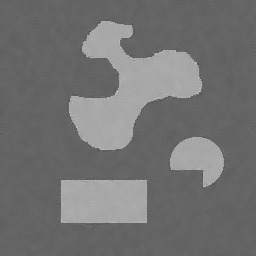
\includegraphics[width = 50mm]{./img/nltroppetit4-2-10.jpg}\\
		\textit{$t=4, r=2, \sigma=10$}\\
	\end{center}
\end{minipage}
\begin{minipage}[c]{0.50\linewidth}
	\begin{center}
		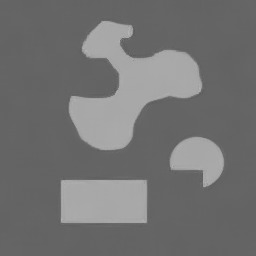
\includegraphics[width = 50mm]{./img/nlassezgrand10-5-10.jpg}\\
		\textit{$t=10, r=5, \sigma=10$}\\
	\end{center}
\end{minipage}\\
\\
\subsection{Estimation du bruit}
Dans le cas de l'implémentation du bruit, et pour se rapprocher des valeurs données en exemple dans le sujet (seuil de 60) nous avons jugé plus pertinent de renvoyer la valeur de l'écart type plutôt que la variance en elle-même ($\sigma = \sqrt{V}$).


\section{Partie II : Comparaison des filtres}
\subsection{Comparaison quantitative}

Les tests suivants ont été effectués sur plusieurs images, présentant un bruit ou une intensité de bruit différente. Les images des différents bruits ont été choisis de manière à avoir une variance uniforme entre les différents types (variance calculée identique pour les trois derniers bruits), permettant ainsi une bonne comparaison.\\

Dans chaque cas le test a été effectué dans le but d'obtenir un PSNR maximal (choix des paramètres en conséquence). C'est pour ce PSNR obtenu que le temps CPU est mesuré. Les temps ainsi mesurés ont été moyennés sur 5 réalisations. Les valeurs renseignées pour le filreNL-Means sont dans l'ordre : $t$ (région), $r$ (patchs), $\sigma$.\\

Image \textit{formes2bb10.pgm}, présentant un faible bruit gaussien (Estimation de bruit : 22.27).

\begin{center}
\begin{tabular}{|l||c|c|c|c|}
\hline
formes2bb10 & Filtre Médian & Filtre Adaptatif & Filtre Bilatéral & Filtre NL-Means \\
& & k=12 & & 10,5,10\\
\hline
Estimation du bruit
&
& 22.82
&
& 22.87\\
\hline
PSNR
&
& 40.85
&
& 40.02\\
\hline
Temps CPU
& 
& 1.002s
&
& 1m20.23s\\
\hline
\end{tabular} 
\end{center}

\vspace{2em}

Image \textit{formes2bb67.pgm}, présentant un fort bruit gaussien (Estimation de bruit : 180.25).

\begin{center}
\begin{tabular}{|l||c|c|c|c|}
\hline
formes2bb67 & Filtre Médian & Filtre Adaptatif & Filtre Bilatéral & Filtre NL-Means\\
& & k=36 & & 10,5,49\\
\hline
Estimation du bruit
&
& 24.98
&
& 26.13\\
\hline
PSNR
&
& 25.02
&
& 27.17\\
\hline
Temps CPU
&
& 3.345s
&
& 1m19.92s\\
\hline
\end{tabular} 
\end{center}

\vspace{2em}

Image \textit{formes2pets5.pgm}, présentant un fort bruit poivre et sel (Estimation de bruit : 150.13).

\begin{center}
\begin{tabular}{|l||c|c|c|c|}
\hline
formes2pets5  & Filtre Médian & Filtre Adaptatif & Filtre Bilatéral & Filtre NL-Means\\
& & k=32 & & 6,4,39\\
\hline
Estimation du bruit
&
& 24.59
&
& 30.90\\
\hline
PSNR
&
& 25.23
&
& 26.15\\
\hline
Temps CPU
&
& 3.321s
&
& 22.897s\\
\hline
\end{tabular} 
\end{center}

\vspace{2em}

Image \textit{formes2sp5.pgm}, présentant un fort bruit speckle (Estimation de bruit : 170.18).

\begin{center}
\begin{tabular}{|l||c|c|c|c|}
\hline
formes2sp5  & Filtre Médian & Filtre Adaptatif & Filtre Bilatéral & Filtre NL-Means \\
& & k=48 & &6,5,91\\
\hline
Estimation du bruit
&
& 23.86
&
& 27.60\\
\hline
PSNR
&
& 23.80
&
& 25.86\\
\hline
Temps CPU
&
& 3.346s
&
& 28.691s\\
\hline
\end{tabular} 
\end{center}

On remarque alors que le filtre NL-Means, bien qu'offrant des résultats très satisfaisants est bien plus long que les autres filtres. Il est possible de diminuer son temps d'éxecution en prenant des régions plus petites (par ex. $t=4$, $r=2$) au prix d'une augmentation du facteur de lissage $\sigma$ et d'un moins bon filtrage (l'ordre de temps est alors inférieur à 10s et se rapproche de ceux obtenus pour les autres filtres).


\vspace{2em}

\subsection{Comparaison qualitative}

Nous avions vu lors du TP précédent que le PSNR permet d'avoir une idée générale mais qu'une estimation visuelle permet de trouver un meilleur compromis entre le bruit persistant et la conservation des contours de l'image. La comparaison visuelle qualitative apparaît donc indispensable.\\

Nous avons choisi l'image \textit{globulesbb25.pgm} afin d'avoir une image présentant plus de critères de comparaison que les formes précédentes (dégradés de couleur, contours, niveaux de couleur...). Cette image présente un bruit gaussien moyen, d'une variance estimée à $54.25$. Les résultats obtenus pour les différents filtres sont les suivants :\\

\noindent
\begin{center}
	\begin{minipage}[c]{0.24\linewidth}
		\begin{center}
			\includegraphics[width = 40mm]{./img/globMedian.jpg}
			\textit{Filtre Médian}
			\textit{$t = , r= , \sigma=$}\
		\end{center}
	\end{minipage}
	\begin{minipage}[c]{0.24\linewidth}
		\begin{center}
			\includegraphics[width = 40mm]{./img/globAdapt.jpg}
			\textit{Filtre Adaptatif}\
			\textit{$K = $}\
		\end{center}
	\end{minipage}
	\begin{minipage}[c]{0.24\linewidth}
		\begin{center}
			\includegraphics[width = 40mm]{./img/globBilat.jpg}
			\textit{Filtre Bilatéral}
			\textit{$t = , r= , \sigma=$}\
		\end{center}
	\end{minipage}
	\begin{minipage}[c]{0.24\linewidth}
		\begin{center}
			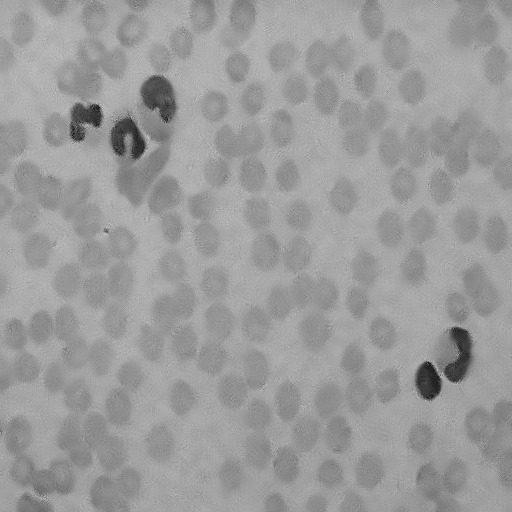
\includegraphics[width = 40mm]{./img/globNLMeans.jpg}
			\textit{Filtre NL-Means}
			\textit{$t = , r= , \sigma=$}\
		\end{center}
	\end{minipage}\\
\end{center}

% Fin section 2 %
\end{document}

% Fin du document LaTeX
